\chapter{Results and Discussion}
\label{ch:results}

This chapter presents and interprets the design-space exploration. It is
organised from the fine grain outward: Section~\ref{sec:res-fu} examines the cost
of hardening individual functional units; Section~\ref{sec:res-full} the cost of
hardening the full datapath; Section~\ref{sec:res-comp} the composition of that
cost in terms of cells, area, and power; Section~\ref{sec:res-timing} the timing
impact; Section~\ref{sec:res-tradeoff} the area--power trade-off;
Section~\ref{sec:res-repl} the replication scenario; and
Section~\ref{sec:res-nodes} the stability of the findings across nodes.
Section~\ref{sec:res-guidelines} distils the results into design guidelines.
Unless stated otherwise, every quantity is the overhead factor relative to the
per-node baseline, as defined in Section~\ref{sec:ex-metrics}.

\section{Per-functional-unit hardening}
\label{sec:res-fu}

Figure~\ref{fig:fu-area} shows the cell-area overhead of hardening each
functional unit individually, for DMR and TMR, at the three nodes;
Figure~\ref{fig:fu-power} shows the corresponding total-power overhead. The
single most important result of the whole study is visible immediately: \emph{the
cost of redundancy is dominated by which unit is hardened, not merely by whether
DMR or TMR is chosen.}

\begin{figure}[htbp]
\centering
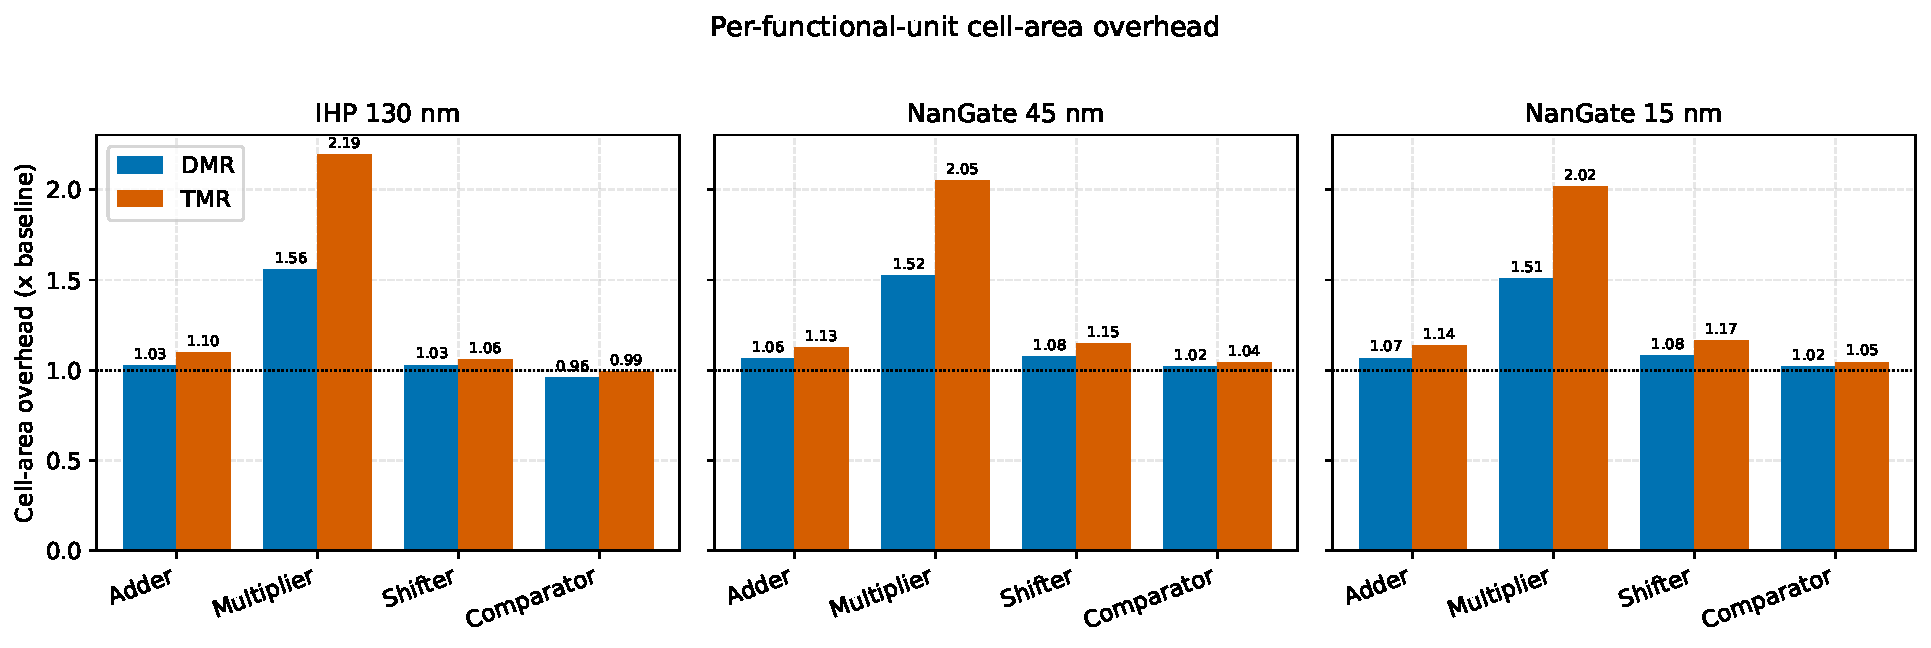
\includegraphics[width=\textwidth]{img/plots/fu_area_overhead.pdf}
\caption{Cell-area overhead of hardening each functional unit individually,
relative to the per-node baseline. The multiplier dominates; the comparator is
almost free. The pattern is essentially identical across the three nodes.}
\label{fig:fu-area}
\end{figure}

\begin{figure}[htbp]
\centering
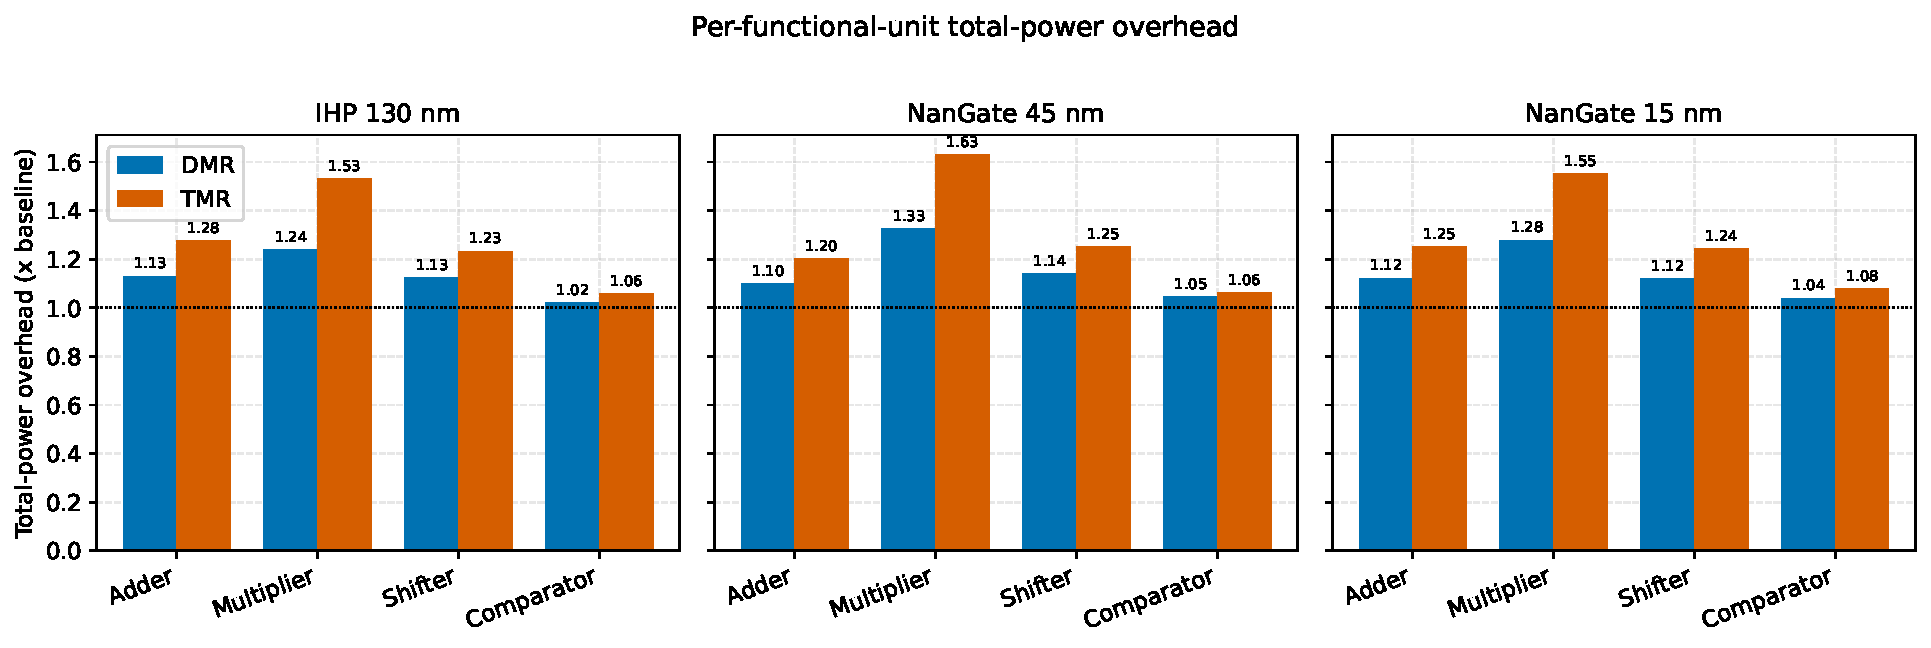
\includegraphics[width=\textwidth]{img/plots/fu_power_overhead.pdf}
\caption{Total-power overhead of hardening each functional unit individually,
relative to the per-node baseline.}
\label{fig:fu-power}
\end{figure}

The \textbf{multiplier} is by far the most expensive unit to protect. At the
mature node, multiplier DMR raises the total cell area to roughly $1.56\times$
the baseline and multiplier TMR to roughly $2.19\times$ --- meaning the
multiplier alone accounts for about half of the entire accelerator's area, so
duplicating it adds about half a baseline and triplicating it adds about a full
baseline. The \textbf{adder} and \textbf{shifter} are moderate and very similar
to each other (DMR around $1.03$--$1.08\times$, TMR around $1.06$--$1.17\times$),
reflecting their comparable, modest size. The \textbf{comparator} is the
cheapest: its DMR and TMR change the total area by only a few percent, and at the
mature node the comparator-DMR area even falls marginally \emph{below} the
baseline ($0.96\times$) --- the logic added is so small that it is lost in the
run-to-run variation of synthesis optimisation. The comparator is the smallest
arithmetic unit and reuses information already produced by the adder, so
protecting it is essentially free.

The same ordering holds for power (Figure~\ref{fig:fu-power}), and the power
overheads remain \emph{smaller} than the area overheads --- multiplier TMR, for
example, costs about $2.19\times$ the area but only about $1.53\times$ the power
at the mature node. The reason is that the duplicated copies are not all
maximally active simultaneously, and a large part of the accelerator's power
(control, mapping, scratchpad interface) is unaffected by datapath redundancy,
so the relative power increase is diluted. Tables~\ref{tab:abs_130nm},
\ref{tab:abs_45nm}, and \ref{tab:abs_15nm} give the underlying absolute numbers
for the three nodes.

\begin{table}[htbp]
\centering
\caption{Synthesis results for the single-core fault-tolerance configurations at IHP 130\,nm. Area is in library units, power in mW, and delay is the critical-path (data-arrival) time in the library time unit.}
\label{tab:abs_130nm}
\small
\begin{tabular}{lrrrrr}
\toprule
Configuration & Cell area & Comb. cells & Seq. cells & Power (mW) & Delay \\
\midrule
Baseline & 361,737 & 32,295 & 1,328 & 20.41 & 4.91 \\
Adder DMR & 371,068 & 32,264 & 1,568 & 23.05 & 5.04 \\
Adder TMR & 396,685 & 33,658 & 1,808 & 26.04 & 4.99 \\
Multiplier DMR & 562,749 & 52,269 & 1,648 & 25.27 & 5.11 \\
Multiplier TMR & 793,544 & 75,388 & 1,968 & 31.24 & 5.14 \\
Shifter DMR & 372,255 & 32,459 & 1,520 & 22.97 & 5.02 \\
Shifter TMR & 382,853 & 32,697 & 1,712 & 25.17 & 5.15 \\
Comparator DMR & 347,479 & 30,652 & 1,392 & 20.83 & 5.08 \\
Comparator TMR & 359,507 & 31,555 & 1,456 & 21.61 & 4.99 \\
Full DMR & 591,559 & 52,962 & 2,144 & 31.36 & 5.21 \\
Full TMR & 871,559 & 78,796 & 2,960 & 42.80 & 5.20 \\
\bottomrule
\end{tabular}
\end{table}

\begin{table}[htbp]
\centering
\caption{Synthesis results for the single-core fault-tolerance configurations at NanGate 45\,nm. Area is in library units, power in mW, and delay is the critical-path (data-arrival) time in the library time unit.}
\label{tab:abs_45nm}
\small
\begin{tabular}{lrrrrr}
\toprule
Configuration & Cell area & Comb. cells & Seq. cells & Power (mW) & Delay \\
\midrule
Baseline & 28,112 & 16,497 & 1,328 & 5.16 & 2.97 \\
Adder DMR & 29,895 & 17,077 & 1,568 & 5.67 & 2.97 \\
Adder TMR & 31,667 & 17,701 & 1,808 & 6.20 & 2.99 \\
Multiplier DMR & 42,867 & 24,816 & 1,648 & 6.84 & 3.02 \\
Multiplier TMR & 57,640 & 33,311 & 1,968 & 8.41 & 3.03 \\
Shifter DMR & 30,262 & 17,698 & 1,520 & 5.88 & 2.94 \\
Shifter TMR & 32,230 & 18,755 & 1,712 & 6.46 & 2.99 \\
Comparator DMR & 28,716 & 16,835 & 1,392 & 5.40 & 2.97 \\
Comparator TMR & 29,303 & 17,188 & 1,456 & 5.48 & 2.99 \\
Full DMR & 47,283 & 26,677 & 2,144 & 8.11 & 2.97 \\
Full TMR & 66,351 & 37,111 & 2,960 & 11.20 & 3.02 \\
\bottomrule
\end{tabular}
\end{table}

\begin{table}[htbp]
\centering
\caption{Synthesis results for the single-core fault-tolerance configurations at NanGate 15\,nm. Area is in library units, power in mW, and delay is the critical-path (data-arrival) time in the library time unit.}
\label{tab:abs_15nm}
\small
\begin{tabular}{lrrrrr}
\toprule
Configuration & Cell area & Comb. cells & Seq. cells & Power (mW) & Delay \\
\midrule
Baseline & 7,254 & 14,199 & 1,328 & 1.69 & 456.39 \\
Adder DMR & 7,746 & 14,812 & 1,568 & 1.90 & 456.39 \\
Adder TMR & 8,238 & 15,458 & 1,808 & 2.11 & 456.40 \\
Multiplier DMR & 10,936 & 20,737 & 1,648 & 2.16 & 460.63 \\
Multiplier TMR & 14,620 & 27,410 & 1,968 & 2.62 & 461.10 \\
Shifter DMR & 7,848 & 15,542 & 1,520 & 1.89 & 454.14 \\
Shifter TMR & 8,452 & 17,060 & 1,712 & 2.10 & 454.14 \\
Comparator DMR & 7,418 & 14,483 & 1,392 & 1.76 & 457.53 \\
Comparator TMR & 7,585 & 14,902 & 1,456 & 1.82 & 455.71 \\
Full DMR & 12,188 & 22,986 & 2,144 & 2.65 & 458.43 \\
Full TMR & 17,136 & 32,251 & 2,960 & 3.59 & 458.38 \\
\bottomrule
\end{tabular}
\end{table}


\section{Full-accelerator hardening}
\label{sec:res-full}

When all four arithmetic units are hardened together, the costs compose almost
additively. Figure~\ref{fig:full} shows the full-accelerator overhead for area,
power, and delay across the three nodes.

\begin{figure}[htbp]
\centering
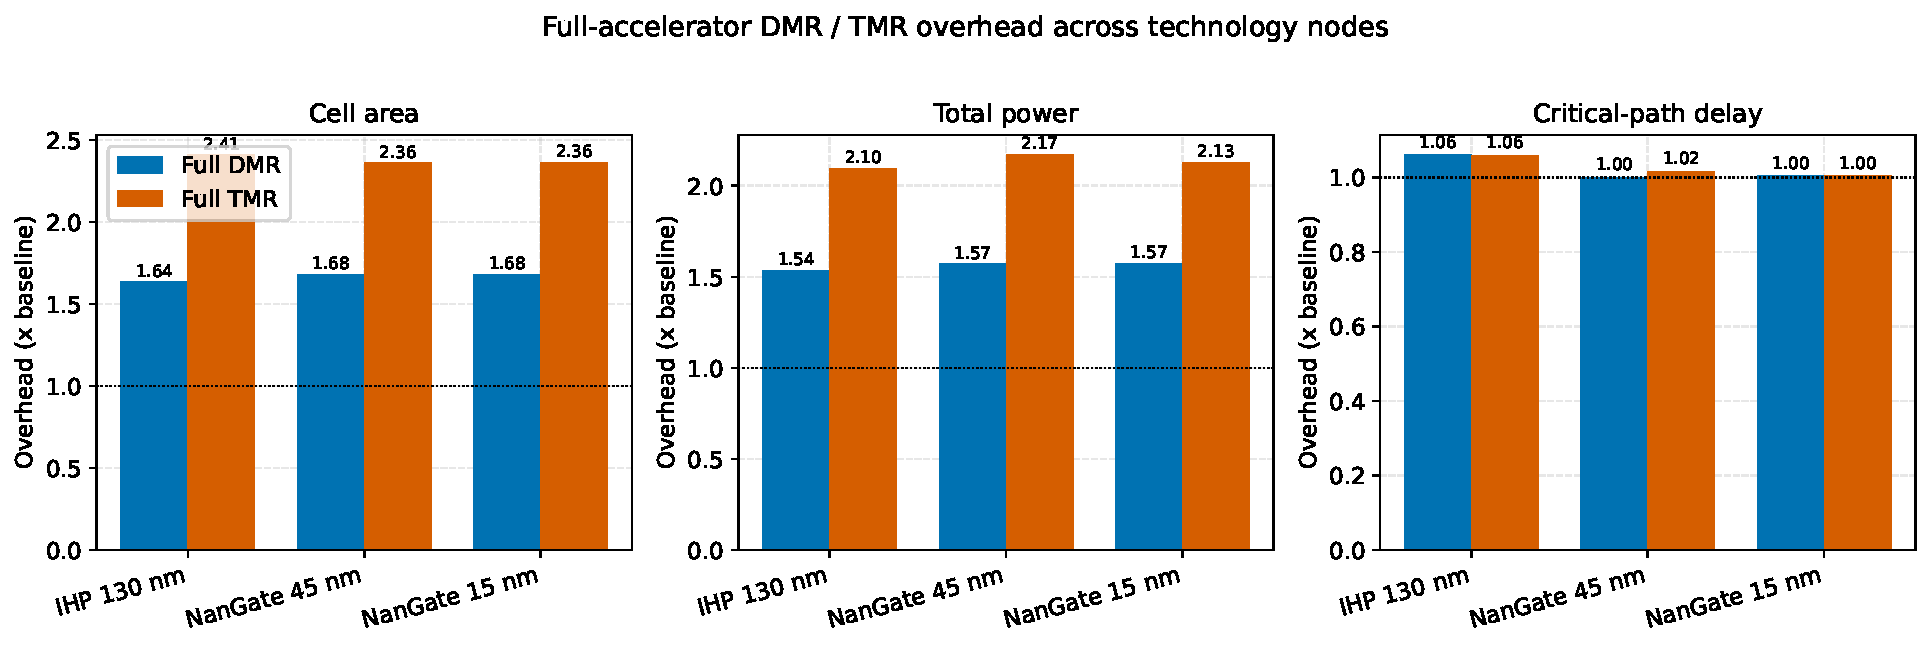
\includegraphics[width=\textwidth]{img/plots/full_overhead.pdf}
\caption{Full-accelerator DMR and TMR overhead --- area, power, and
critical-path delay --- across the three technology nodes.}
\label{fig:full}
\end{figure}

Full DMR costs about $1.64$--$1.68\times$ the baseline area and full TMR about
$2.36$--$2.41\times$, consistently across all three nodes. It is worth dwelling on why
these are \emph{below} the naive ``$2\times$ for DMR, $3\times$ for TMR''
expectation. That naive expectation would hold only if the \emph{entire} design
were duplicated or triplicated. Here, only the arithmetic functional units are
replicated; the mapping layer, the pipeline and FU controllers, the exception
unit, and the scratchpad interface remain single-copy. Since these unhardened
parts constitute a substantial fraction of the baseline, the overall multiplier
is pulled well below $2\times$ and $3\times$. This is a direct, quantitative
benefit of \emph{fine-grained} hardening: by protecting only the datapath, the
designer avoids paying to triplicate logic that may not need it.

The full-accelerator power overhead is about $1.54$--$1.57\times$ for DMR and
about $2.10$--$2.17\times$ for TMR --- still below the corresponding area factors,
for the same dilution reason as in Section~\ref{sec:res-fu}, though the gap
between the area and power penalties is narrower for the full datapath than for
any single unit, because hardening every unit activates a larger share of the
added logic.

\section{Composition of the overhead}
\label{sec:res-comp}

To understand \emph{where} the extra cost goes, Figures~\ref{fig:area-comp} and
\ref{fig:power-comp} decompose area and power by category for every Scenario~A
configuration at the mature node (the finer nodes behave analogously), and
Figure~\ref{fig:cells} shows the combinational and sequential cell counts.

\begin{figure}[htbp]
\centering
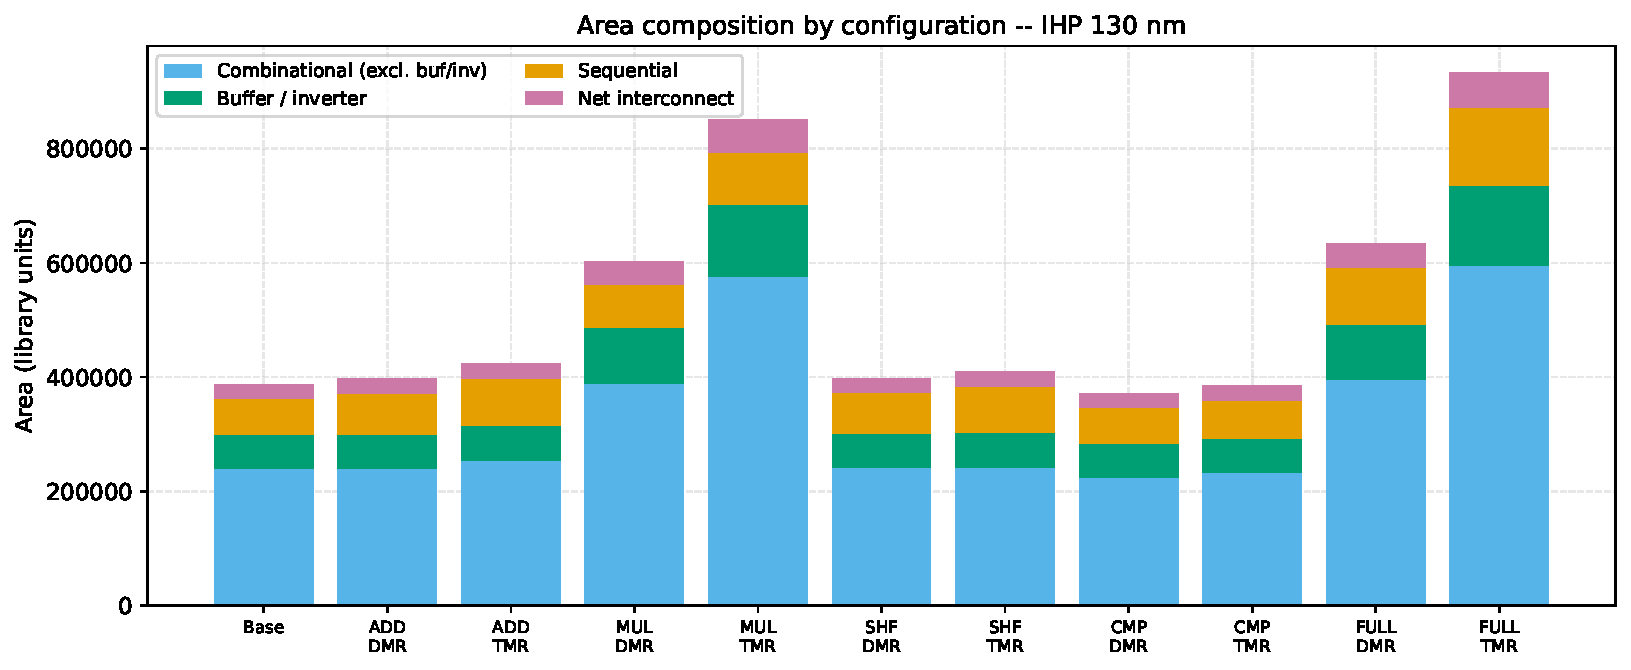
\includegraphics[width=\textwidth]{img/plots/area_composition_130nm.pdf}
\caption{Area composition by configuration at IHP 130\,nm: combinational,
buffer/inverter, sequential, and net-interconnect area. Redundancy adds
predominantly combinational logic.}
\label{fig:area-comp}
\end{figure}

\begin{figure}[htbp]
\centering
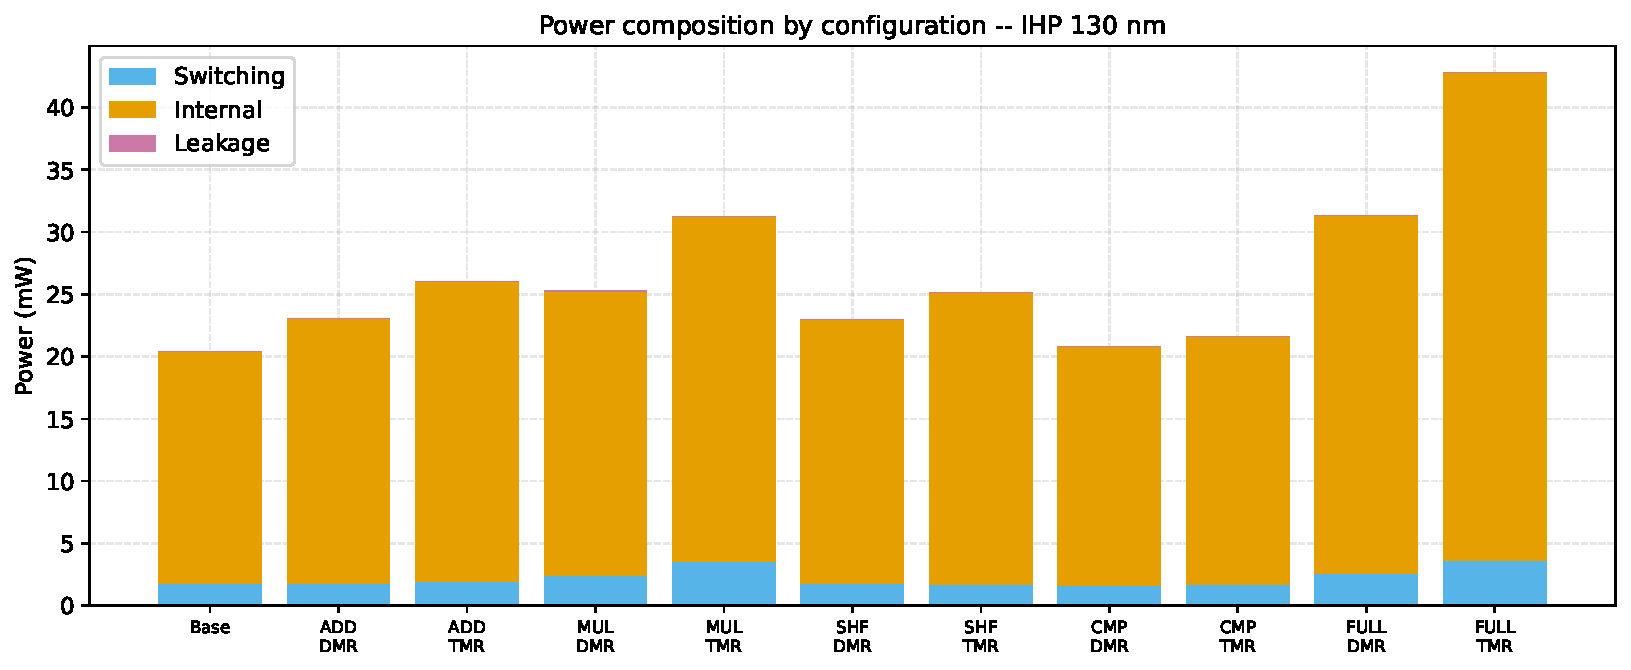
\includegraphics[width=\textwidth]{img/plots/power_composition_130nm.pdf}
\caption{Power composition by configuration at IHP 130\,nm: switching, internal,
and leakage power.}
\label{fig:power-comp}
\end{figure}

\begin{figure}[htbp]
\centering
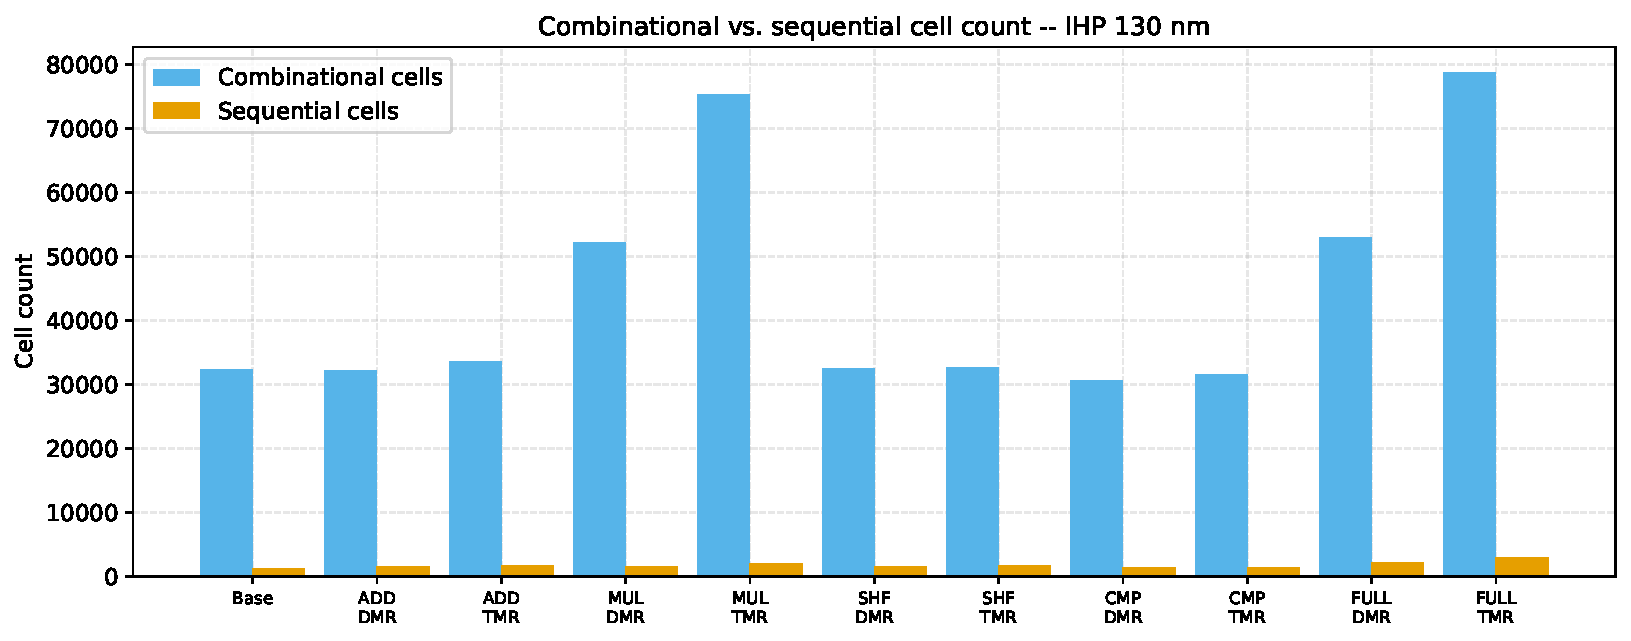
\includegraphics[width=\textwidth]{img/plots/cell_counts_130nm.pdf}
\caption{Combinational versus sequential cell counts by configuration at IHP
130\,nm. The growth is overwhelmingly in combinational cells.}
\label{fig:cells}
\end{figure}

The decomposition confirms the intuition behind the wrappers. The extra area is
overwhelmingly \emph{combinational}: the duplicated/triplicated functional-unit
logic plus the comparison/voter arrays. The sequential-cell count barely moves
for the lighter units and grows only where the protected unit is itself
pipelined and large (the multiplier). This matters for reliability reasoning:
the redundancy is concentrated exactly where transient errors in combinational
arithmetic would otherwise propagate silently. The power decomposition tells the
same story --- the increase is concentrated in the switching and internal power
of the added combinational logic, with leakage scaling roughly in proportion to
the added cells.

\subsection{Composition at the finer nodes}
\label{sec:res-comp-nodes}

The same decomposition holds at the mainstream and advanced nodes, confirming
that it reflects the structure of the redundancy rather than a quirk of one
library. Figures~\ref{fig:area-comp-45} and \ref{fig:area-comp-15} show the area
composition at NanGate 45\,nm and 15\,nm; Figures~\ref{fig:power-comp-45} and
\ref{fig:power-comp-15} the power composition; and
Figures~\ref{fig:cells-45} and \ref{fig:cells-15} the cell counts. In every case
the redundancy overhead is dominated by added combinational cells, the sequential
count grows materially only for the multiplier, and the multiplier and
full-datapath configurations stand out as the tall bars --- exactly as at the
mature node. The one systematic difference is the relative weight of leakage in
the power stacks, which grows at the finer nodes, consistent with the
well-known increase of static power in advanced CMOS; this shifts the balance of
\emph{where} the redundancy power goes but not the overall ordering of the
configurations.

\begin{figure}[htbp]
\centering
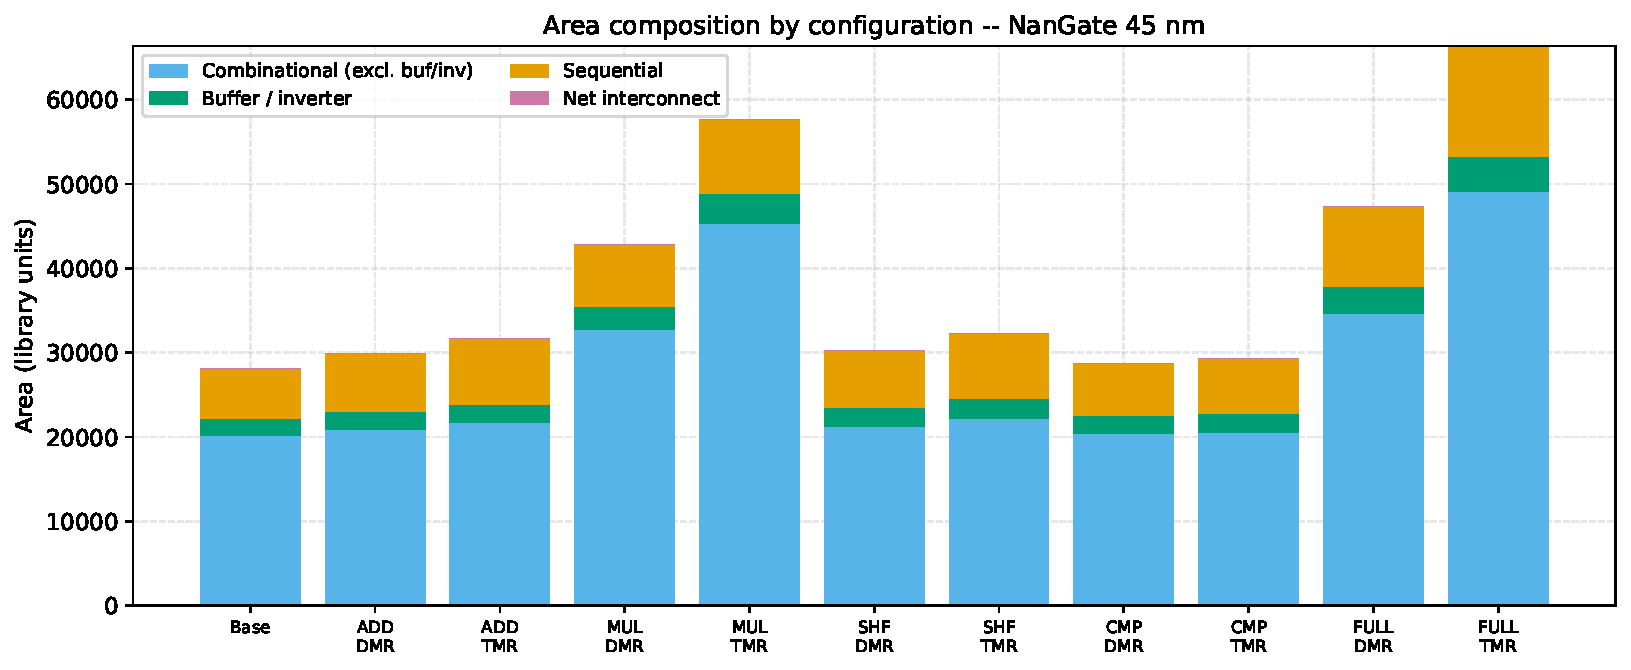
\includegraphics[width=\textwidth]{img/plots/area_composition_45nm.pdf}
\caption{Area composition by configuration at NanGate 45\,nm.}
\label{fig:area-comp-45}
\end{figure}

\begin{figure}[htbp]
\centering
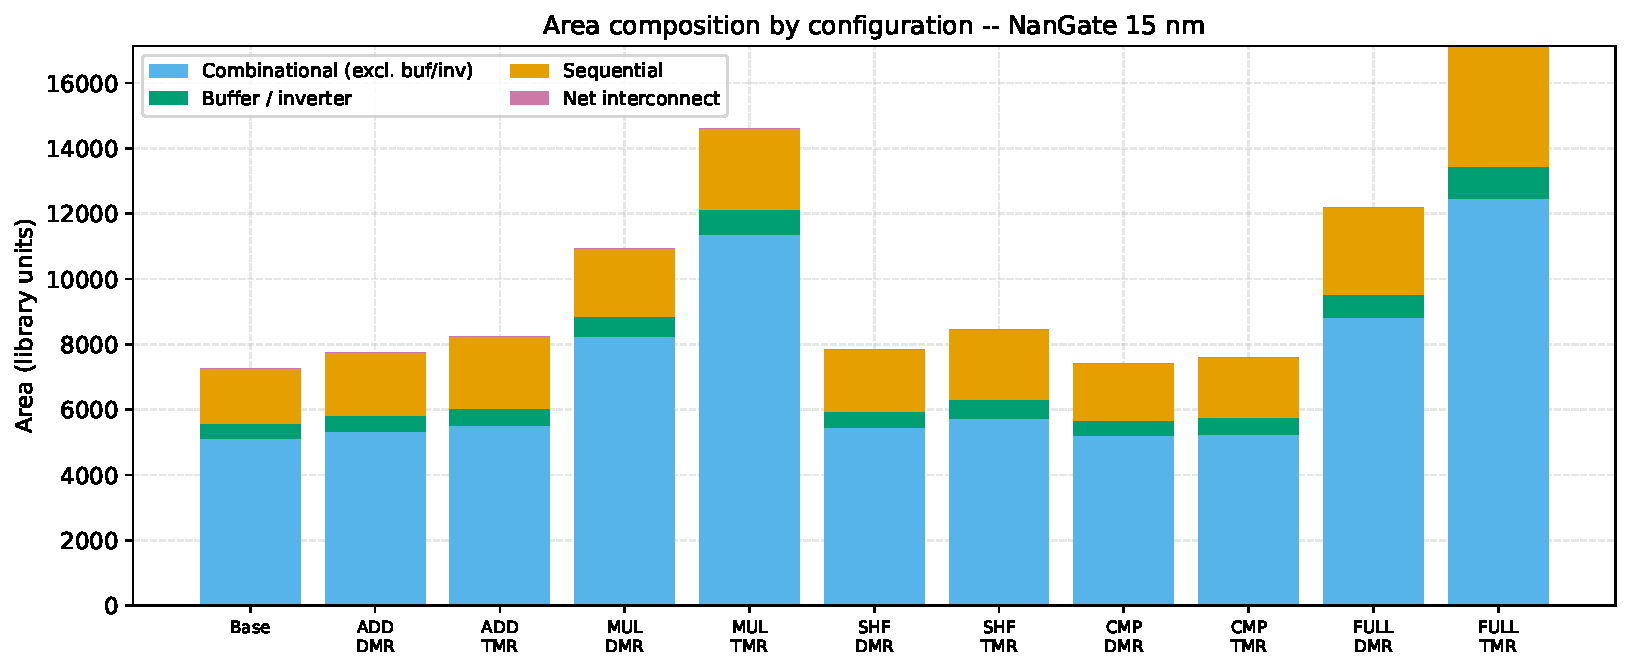
\includegraphics[width=\textwidth]{img/plots/area_composition_15nm.pdf}
\caption{Area composition by configuration at NanGate 15\,nm.}
\label{fig:area-comp-15}
\end{figure}

\begin{figure}[htbp]
\centering
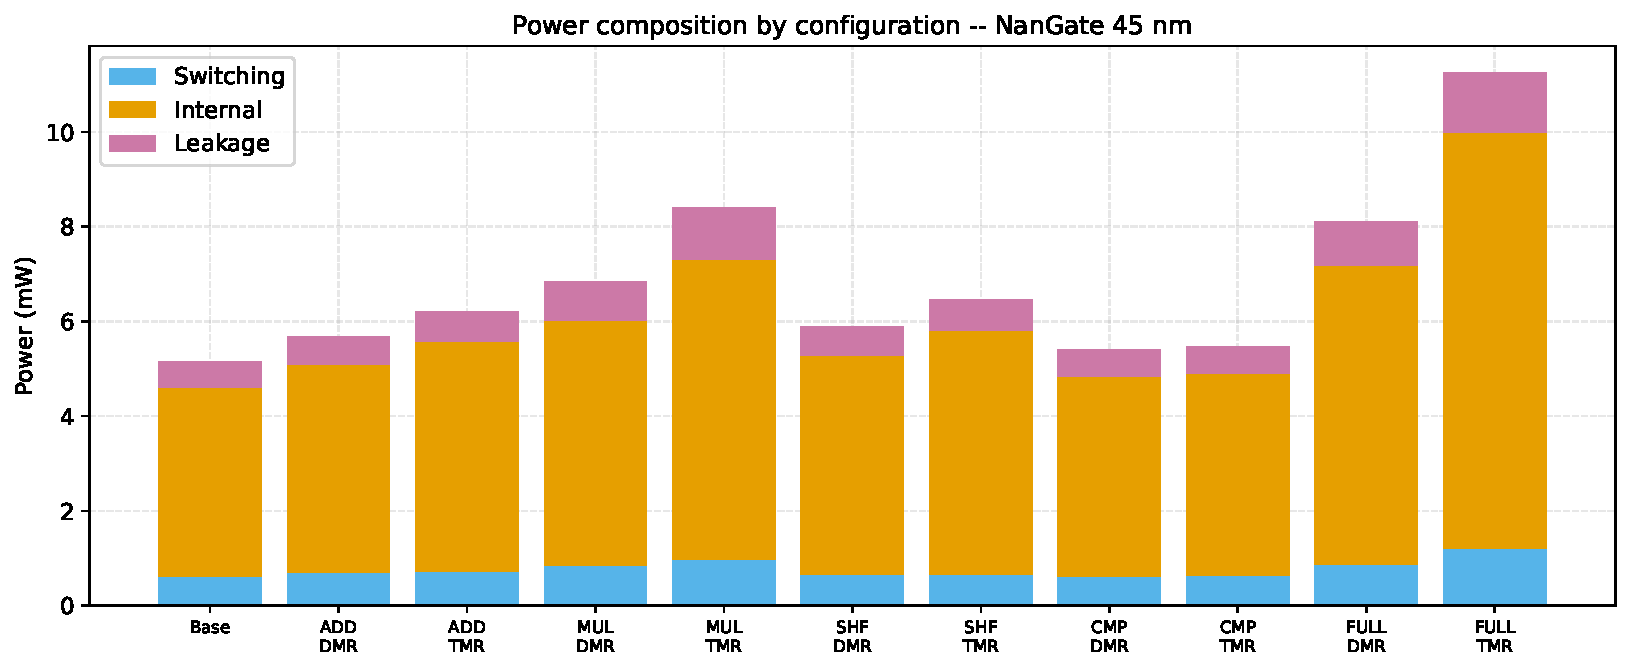
\includegraphics[width=\textwidth]{img/plots/power_composition_45nm.pdf}
\caption{Power composition by configuration at NanGate 45\,nm.}
\label{fig:power-comp-45}
\end{figure}

\begin{figure}[htbp]
\centering
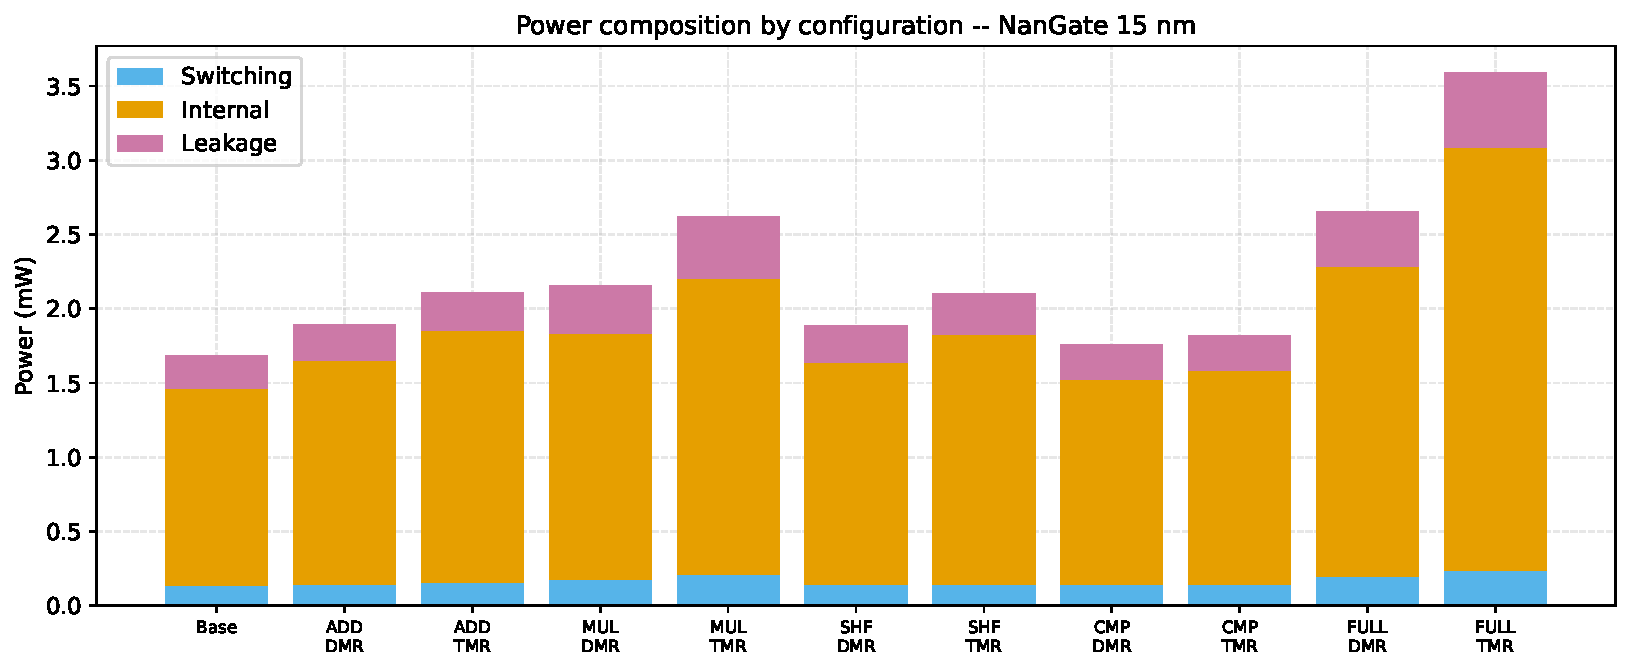
\includegraphics[width=\textwidth]{img/plots/power_composition_15nm.pdf}
\caption{Power composition by configuration at NanGate 15\,nm. Leakage takes a
visibly larger share of the total than at the mature node.}
\label{fig:power-comp-15}
\end{figure}

\begin{figure}[htbp]
\centering
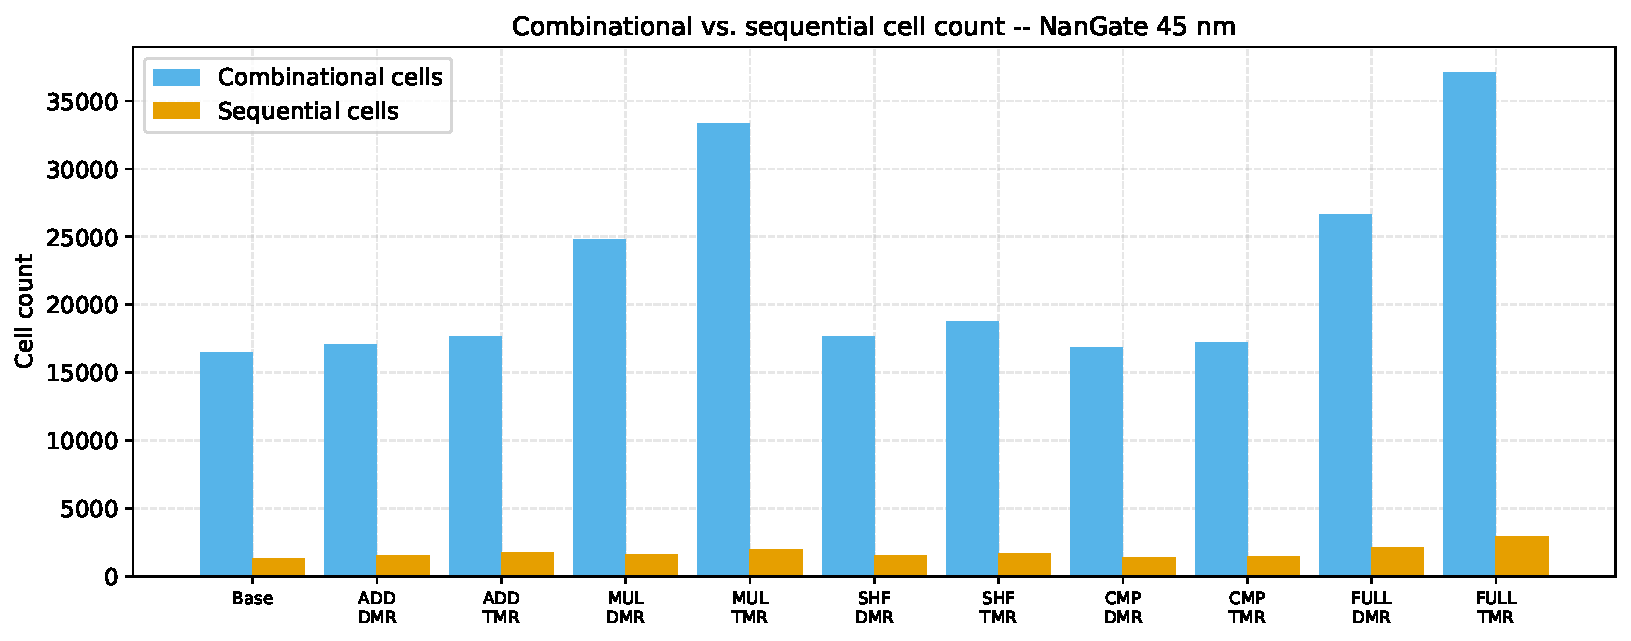
\includegraphics[width=\textwidth]{img/plots/cell_counts_45nm.pdf}
\caption{Combinational versus sequential cell counts at NanGate 45\,nm.}
\label{fig:cells-45}
\end{figure}

\begin{figure}[htbp]
\centering
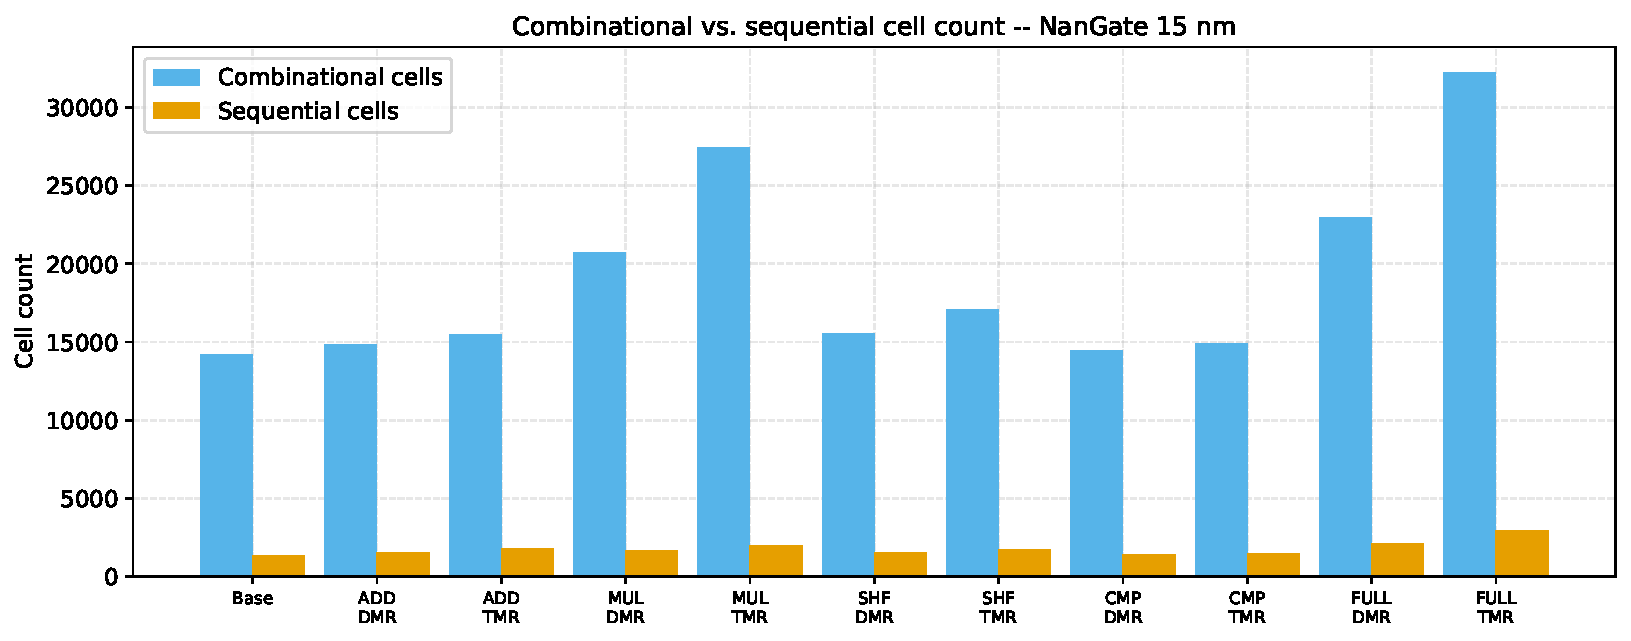
\includegraphics[width=\textwidth]{img/plots/cell_counts_15nm.pdf}
\caption{Combinational versus sequential cell counts at NanGate 15\,nm.}
\label{fig:cells-15}
\end{figure}

\section{Timing impact}
\label{sec:res-timing}

A central question for any redundancy scheme is whether it slows the design down.
The right-hand panel of Figure~\ref{fig:full} answers it: the critical-path delay
is only \emph{mildly} affected by redundancy. The overhead is largest at the
mature node --- about $1.06\times$ for both full DMR and full TMR --- and shrinks
at the finer nodes, to roughly $1.0$--$1.02\times$ at the mainstream node and
essentially $1.00\times$ at the advanced node. The per-unit delay overheads are
even smaller, and a few configurations land marginally below $1.00$, within the
noise of the timing analysis.

This is consistent with what the architecture predicts. The DMR comparator and
the TMR voter are shallow combinational layers --- a few gates deep --- placed on
the functional-unit outputs, while the accelerator's true critical path runs
through other, deeper logic (such as the address arithmetic in the
exception/control path). The voter therefore only occasionally lengthens the
critical path, and then only slightly: hardening every unit (full DMR/TMR) adds a
voter layer to more outputs and so produces the largest --- but still small ---
delay increase, most visibly at the mature node where the baseline path is
longest in absolute terms.

The practical implication is significant: across all three nodes, \emph{the
designer buys fault tolerance with area and power at a delay cost of at most a
few percent}, which removes one of the usual objections to modular redundancy in
high-throughput datapaths.

\section{Area--power trade-off}
\label{sec:res-tradeoff}

Figure~\ref{fig:tradeoff} plots, for the mature node, every Scenario~A
configuration in the area-overhead/power-overhead plane. The configurations form
a clear frontier from the cheap comparator points near the baseline, through the
adder and shifter, to the expensive multiplier and full-datapath points. DMR
points (squares) always sit below and to the left of the corresponding TMR points
(triangles): DMR delivers detection at roughly half the marginal cost of the
masking that TMR provides. The figure is a compact decision aid --- a designer
with a fixed area or power budget can read off which units can be afforded.

\begin{figure}[htbp]
\centering
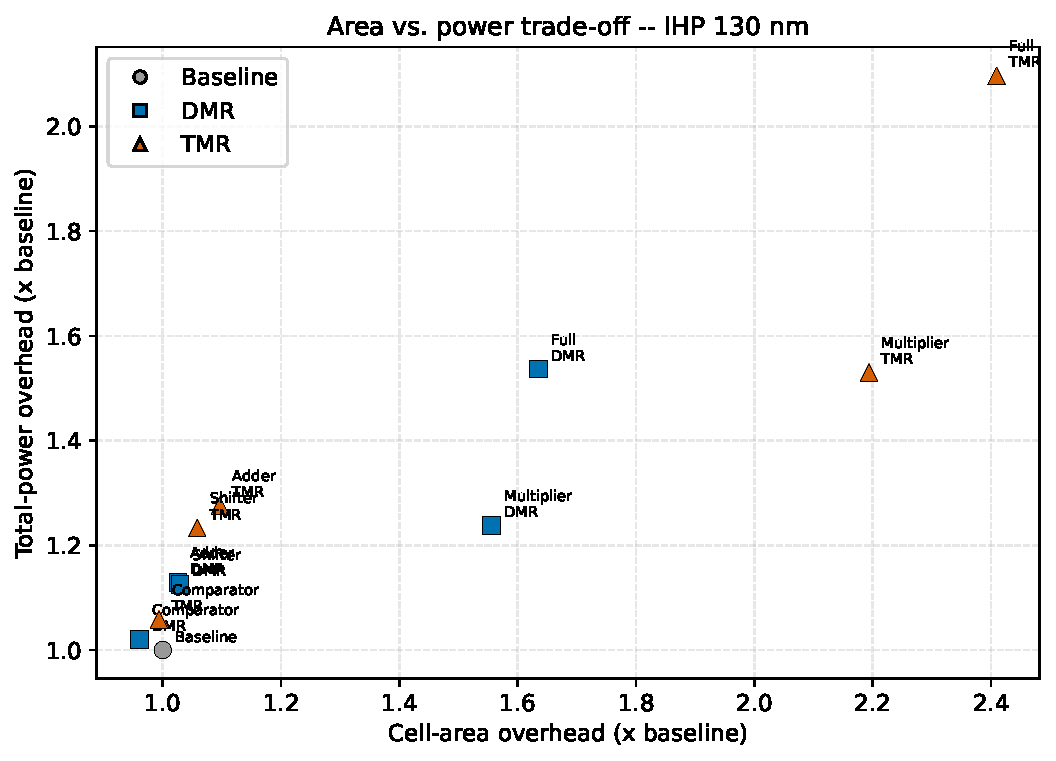
\includegraphics[width=0.78\textwidth]{img/plots/tradeoff_130nm.pdf}
\caption{Area versus power overhead for every single-core configuration at IHP
130\,nm. DMR (squares) consistently dominates TMR (triangles) in cost; the
multiplier and full-datapath points define the expensive end of the frontier.}
\label{fig:tradeoff}
\end{figure}

The same frontier reappears at the other two nodes
(Figures~\ref{fig:tradeoff-45} and \ref{fig:tradeoff-15}): although the absolute
power and area scales differ, the \emph{shape} of the trade-off --- comparator
cheapest, multiplier and full datapath most expensive, DMR dominating TMR --- is
preserved, reinforcing that the decision aid is technology-independent.

\begin{figure}[htbp]
\centering
\begin{subfigure}[t]{0.49\textwidth}
\centering
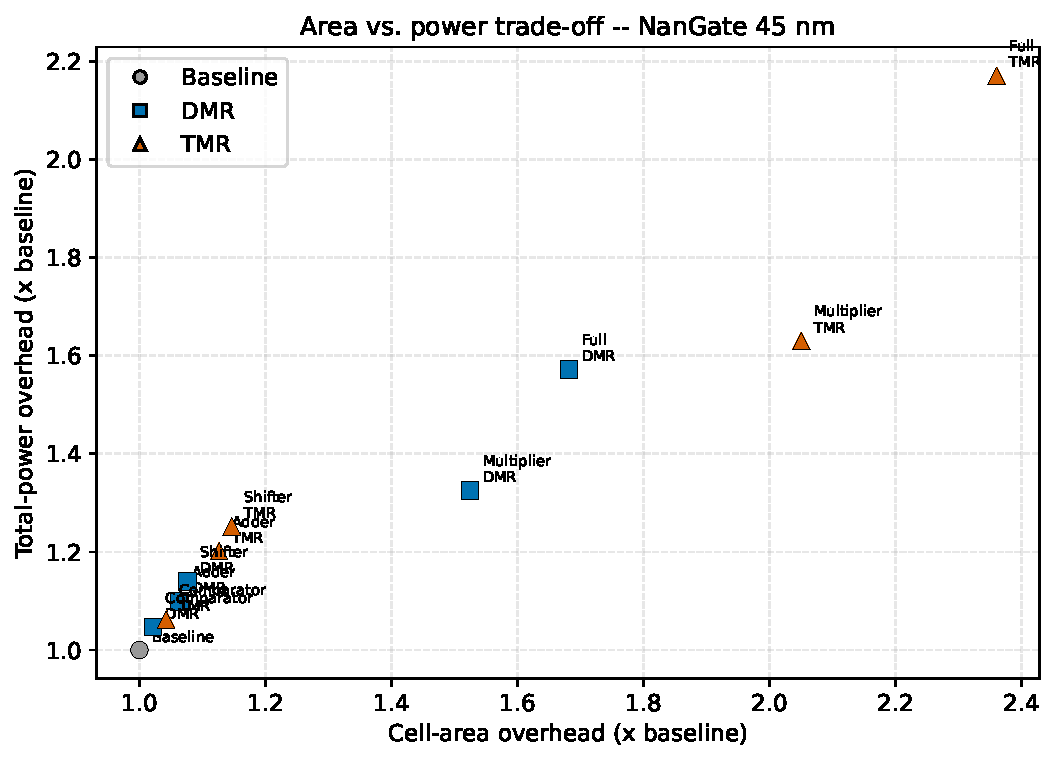
\includegraphics[width=\textwidth]{img/plots/tradeoff_45nm.pdf}
\caption{NanGate 45\,nm.}
\label{fig:tradeoff-45}
\end{subfigure}
\hfill
\begin{subfigure}[t]{0.49\textwidth}
\centering
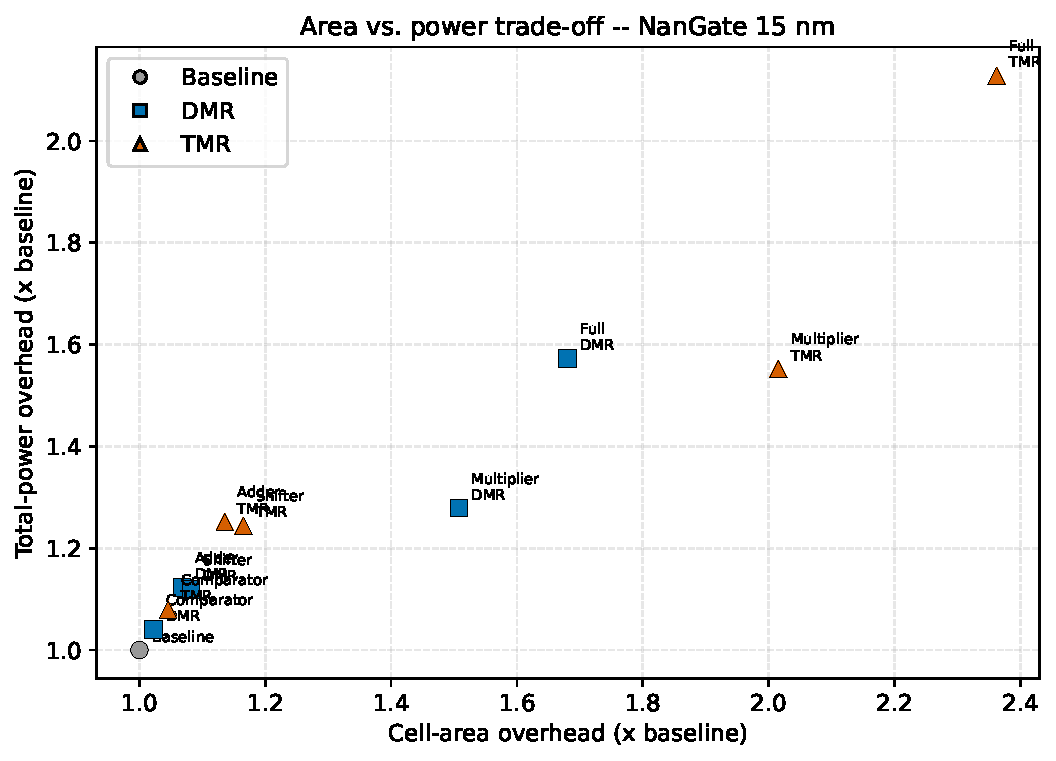
\includegraphics[width=\textwidth]{img/plots/tradeoff_15nm.pdf}
\caption{NanGate 15\,nm.}
\label{fig:tradeoff-15}
\end{subfigure}
\caption{Area versus power trade-off at the mainstream and advanced nodes. The
frontier has the same shape as at the mature node (Figure~\ref{fig:tradeoff}).}
\label{fig:tradeoff-fine}
\end{figure}

The absolute cell areas behind these ratios are shown, per node, in
Figure~\ref{fig:abs-area}; the shapes are identical across nodes even though the
vertical scales differ by orders of magnitude, which is the clearest possible
demonstration that the \emph{relative} cost structure is a property of the
architecture rather than of any one technology.

\begin{figure}[htbp]
\centering
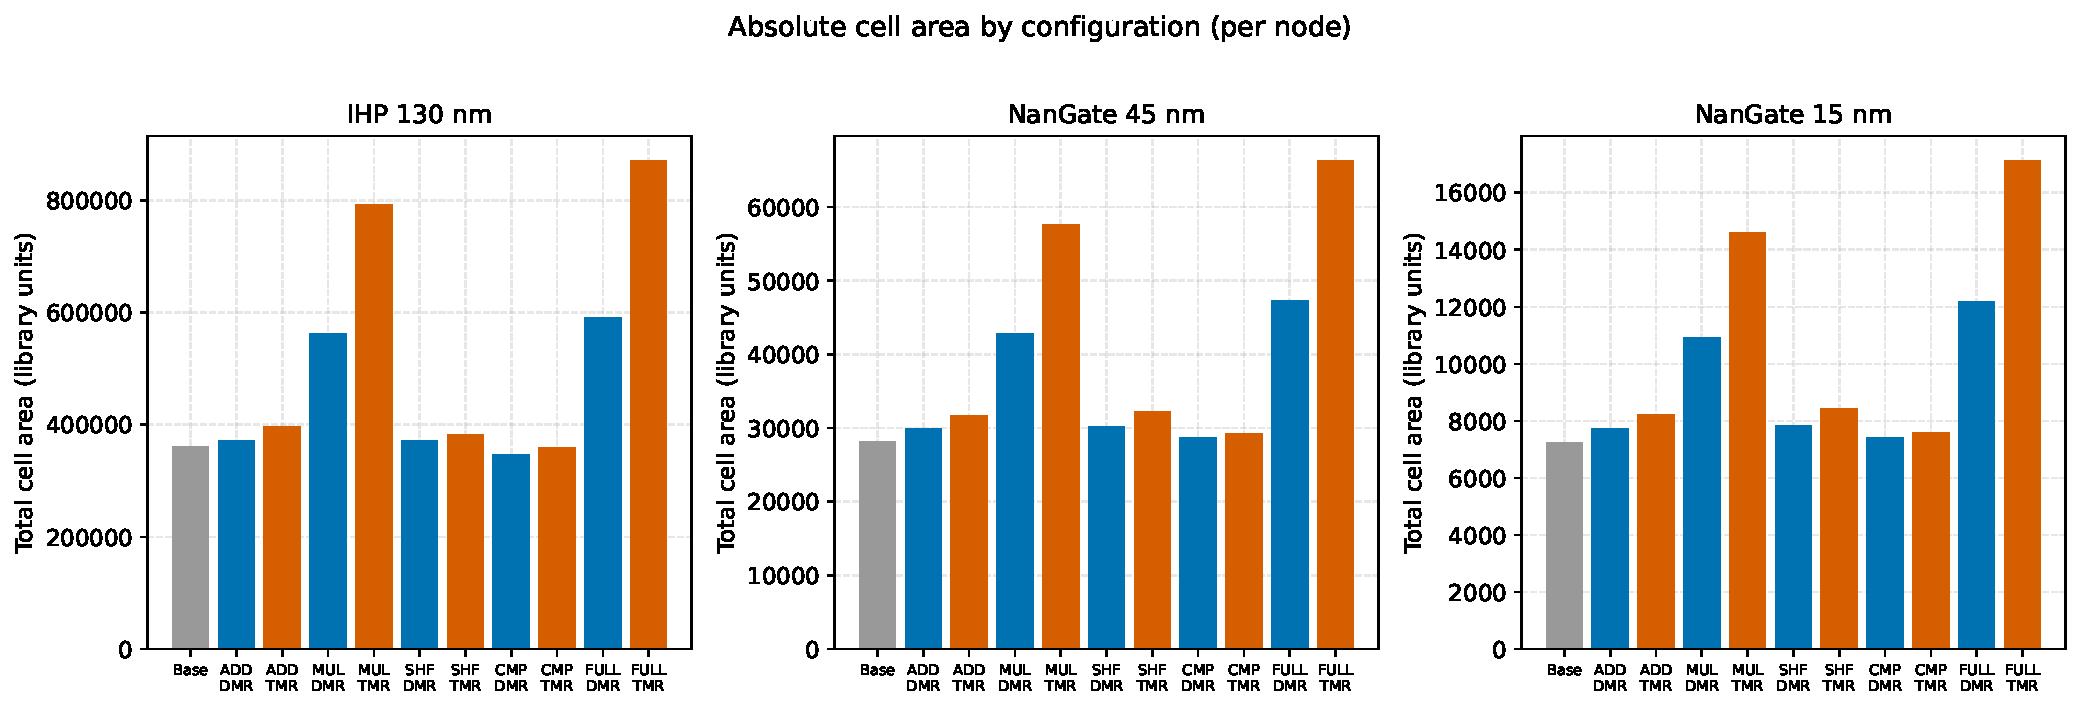
\includegraphics[width=\textwidth]{img/plots/absolute_area.pdf}
\caption{Absolute total cell area by configuration at each node (note the
differing vertical scales). The relative pattern is invariant across nodes.}
\label{fig:abs-area}
\end{figure}

\section{Replication-based redundancy}
\label{sec:res-repl}

Scenario~B evaluates the alternative regime in which the accelerator is already
replicated into three lanes for throughput, and redundancy is obtained by voting
the lanes in the mapping layer. Table~\ref{tab:replication} and
Figure~\ref{fig:repl} report the results.

\begin{table}[htbp]
\centering
\caption{Replication-based redundancy (Scenario~B): three-lane accelerator with voting inserted in the mapping unit. Cell area is given in library units and also normalised to the single-core baseline. Adding voting changes the area only marginally relative to the replicated baseline.}
\label{tab:replication}
\small
\begin{tabular}{llrr}
\toprule
Node & Configuration & Cell area & $\times$ single-core \\
\midrule
IHP 130\,nm & Replicated baseline (3 lanes) & 1,011,568 & 2.80 \\
IHP 130\,nm & Replicated + DMR voting & 950,085 & 2.63 \\
IHP 130\,nm & Replicated + TMR voting & 938,713 & 2.60 \\
\midrule
NanGate 45\,nm & Replicated baseline (3 lanes) & 84,179 & 2.99 \\
NanGate 45\,nm & Replicated + DMR voting & 84,401 & 3.00 \\
NanGate 45\,nm & Replicated + TMR voting & 84,315 & 3.00 \\
\midrule
NanGate 15\,nm & Replicated baseline (3 lanes) & 21,752 & 3.00 \\
NanGate 15\,nm & Replicated + DMR voting & 21,954 & 3.03 \\
NanGate 15\,nm & Replicated + TMR voting & 22,161 & 3.06 \\
\bottomrule
\end{tabular}
\end{table}


\begin{figure}[htbp]
\centering
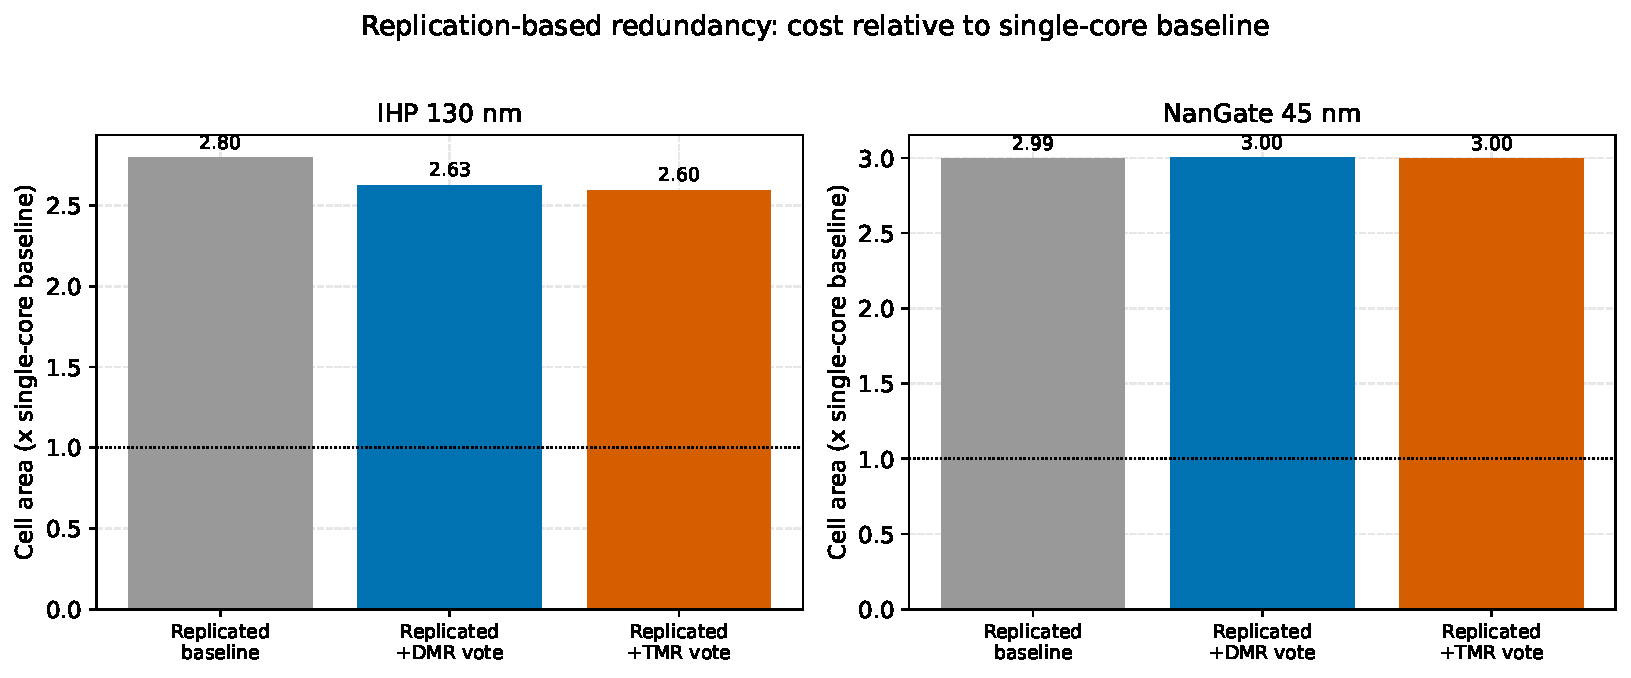
\includegraphics[width=\textwidth]{img/plots/replication_area.pdf}
\caption{Cost of replication-based redundancy relative to the single-core
baseline. The three-lane datapath itself costs roughly $3\times$; adding DMR or
TMR voting on top of it changes the area only marginally.}
\label{fig:repl}
\end{figure}

Two facts stand out. First, the replicated baseline already costs about
$2.8$--$3.0\times$ the single-core baseline --- essentially the unavoidable price
of three lanes. Second, and more interestingly, \emph{adding voting on top of
replication is almost free}: at the mainstream node the replicated-plus-DMR and
replicated-plus-TMR areas sit within a fraction of a percent of the replicated
baseline, and at the advanced node they add only about one to two percent. At the
mature node the voting variants even synthesise slightly \emph{smaller} than the
plain replicated baseline ($2.60$--$2.63\times$ versus $2.80\times$), which is a
clear sign that the marginal logic added by voting is below the noise floor of
synthesis optimisation --- the optimiser simply restructures the large replicated
datapath differently between runs. In every case the message is the same: because
the expensive datapath copies already exist for throughput, only the thin
comparison/voter logic in the mapping layer is genuinely new. The lesson is that
the economics of redundancy depend strongly on context: building TMR from scratch
costs about $2.4\times$ (Section~\ref{sec:res-full}), but \emph{reusing}
replication that is already present for performance turns masking into a
negligible add-on.

\section{Stability across technology nodes}
\label{sec:res-nodes}

Table~\ref{tab:overhead} collects the area and power overheads of every
single-core configuration at all three nodes side by side, and
Figure~\ref{fig:node-summary} tracks the full-accelerator overheads across nodes.

\begin{table}[htbp]
\centering
\caption{Cell-area and total-power overhead of each single-core fault-tolerance configuration, normalised to the per-node baseline ($\times$ baseline). Values are remarkably stable across the three technology nodes.}
\label{tab:overhead}
\small
\begin{tabular}{lrrrrrr}
\toprule
 & \multicolumn{2}{c}{IHP 130\,nm} & \multicolumn{2}{c}{NanGate 45\,nm} & \multicolumn{2}{c}{NanGate 15\,nm} \\
\cmidrule(lr){2-3} \cmidrule(lr){4-5} \cmidrule(lr){6-7}
Configuration & Area & Power & Area & Power & Area & Power \\
\midrule
Adder DMR & 1.03 & 1.13 & 1.06 & 1.10 & 1.07 & 1.12 \\
Adder TMR & 1.10 & 1.28 & 1.13 & 1.20 & 1.14 & 1.25 \\
Multiplier DMR & 1.56 & 1.24 & 1.52 & 1.33 & 1.51 & 1.28 \\
Multiplier TMR & 2.19 & 1.53 & 2.05 & 1.63 & 2.02 & 1.55 \\
Shifter DMR & 1.03 & 1.13 & 1.08 & 1.14 & 1.08 & 1.12 \\
Shifter TMR & 1.06 & 1.23 & 1.15 & 1.25 & 1.17 & 1.24 \\
Comparator DMR & 0.96 & 1.02 & 1.02 & 1.05 & 1.02 & 1.04 \\
Comparator TMR & 0.99 & 1.06 & 1.04 & 1.06 & 1.05 & 1.08 \\
Full DMR & 1.64 & 1.54 & 1.68 & 1.57 & 1.68 & 1.57 \\
Full TMR & 2.41 & 2.10 & 2.36 & 2.17 & 2.36 & 2.13 \\
\bottomrule
\end{tabular}
\end{table}


\begin{figure}[htbp]
\centering
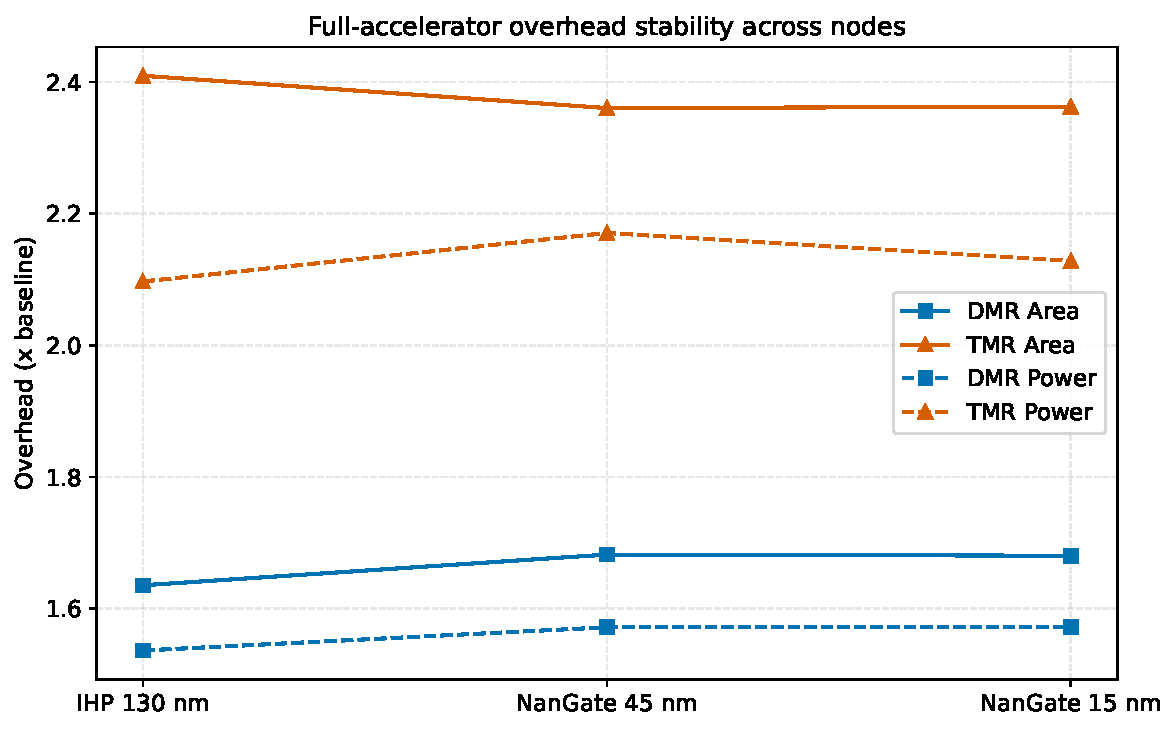
\includegraphics[width=0.72\textwidth]{img/plots/node_summary.pdf}
\caption{Full-accelerator area and power overheads tracked across the three
nodes. The lines are almost flat, showing that the cost of redundancy is a
stable architectural property.}
\label{fig:node-summary}
\end{figure}

The overheads are remarkably consistent: the area factors vary by at most a few
percent across a technology range spanning from 130\,nm down to 15\,nm. This
stability is the second major result of the study. It means that the design
guidelines derived here are not tied to a particular library: a designer can
estimate the cost of a given hardening choice on a new node directly from these
factors, with confidence that the architecture-level ratios will carry over. The
small deviations that do appear --- chiefly the slightly higher power and delay
overheads at the advanced node --- are consistent with the finer node's more
balanced cell/wire delays and its different leakage profile, and do not change
the qualitative picture.

\section{Design guidelines}
\label{sec:res-guidelines}

The results support a compact set of guidelines for hardening a SIMD vector
accelerator of this kind:

\begin{enumerate}
  \item \textbf{Spend the budget on the multiplier last, the comparator first.}
        Because the multiplier dominates the cost of any scheme that includes it,
        and the comparator is almost free, a graceful hardening path is to
        protect the cheap units first and add multiplier protection only when the
        reliability requirement justifies its large area cost.
  \item \textbf{Use DMR for detection, TMR for masking, and choose by system
        need.} DMR roughly halves the marginal cost of TMR while still catching
        errors; if the system can respond to an error flag (retry, rollback, safe
        state), DMR is the economical choice. Reserve TMR for units whose output
        must remain correct without interruption.
  \item \textbf{Harden at fine granularity to avoid over-paying.} Full-datapath
        TMR costs about $2.4\times$ rather than $3\times$ precisely because the
        non-datapath logic is left single-copy; selective hardening lets the
        designer push this saving further.
  \item \textbf{Exploit existing replication.} If the accelerator is already
        replicated for throughput, obtain reliability by voting the existing
        lanes --- the marginal cost is small compared with building redundancy
        anew.
  \item \textbf{Add in-field monitoring freely.} The IJTAG instrumentation costs
        at most a couple of percent (Chapter~\ref{ch:ijtag}) and is independent
        of the redundancy choice, so observability can be combined with any
        hardening configuration without materially changing its cost.
  \item \textbf{Trust the ratios across nodes.} The overhead factors are stable
        across the studied process range, so they can be reused to estimate cost
        on other nodes.
\end{enumerate}
